\chapter{Application}\label{chap:application}
In order to create a robust system, two solutions are proposed. The first utilizes the fact that a person faces 
the same direction their waist faces. So we create a plane between three fixed 
points, the center hip $\vec{c}$, the left $\vec{l}$ and the right hips $\vec{r}$. A normal vector \N was created 
from this plane in order to allow the program to recognize where the person is 
facing.

\begin{figure}[!htbp]
\centering
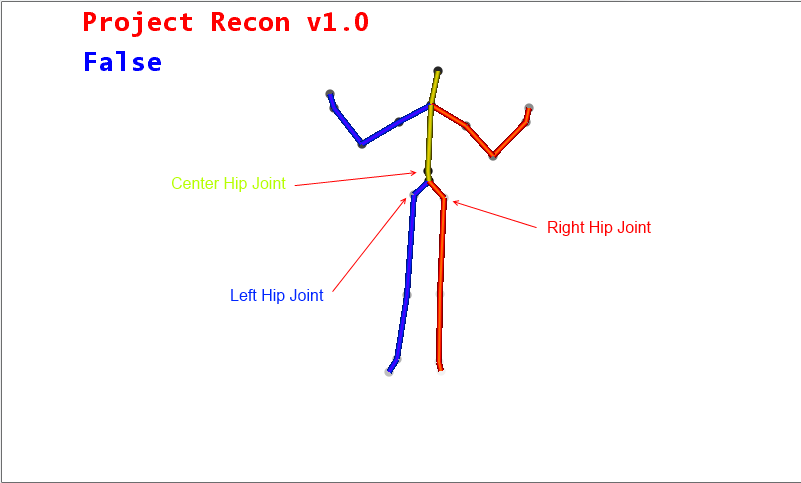
\includegraphics[width=1\textwidth]{images/skeleton_frame3.png}
\caption{In the figure the three joints are pointed out and named}
\label{skeletonframe3}
\end{figure}

To calculate the normal vector, we subtract the right and left hip joints from 
the center hip joint and then we calculate the cross product of the two 
subtractions.
\\
\\
$\vec{N}$ = ($\vec{r}$ - $\vec{c}$) $\times$ ($\vec{l}$ - $\vec{c}$)
\\
\\
We then calculate the normal by using the Normalize method.
\begin{verbatim}
var dir = Vector3.Cross(rhip - chip, lhip - chip);
var norm = Vector3.Normalize(dir);
\end{verbatim}
As the person turns, the normal vector will be used as a reference to calculate the angle between it and the Z axis. This will allow us to rotate the skeleton so that it will be always facing the Kinect. Recognition will then take place.
\\
\\
Kinect has another problem, which is that it cannot diffrentiate between a user giving it his face or his back. In other words, a user's left and right are swaped if the user is giving the Kinect his back.

%put an image to make it better understandable

The normal vector calculation approach will reswap the left joints with the right joints when the \N is on the negative Z axis. 
However, here another problem emerges. When the swap takes place, an error occurs. Mainly, the programmer can not 
edit the value of the position of the joints. The value is read from the skeleton 
stream of the Kinect. In order to resolve this, an avatar skeleton needs to be 
created, littleGuy. littleGuy is an array of SkeletonPoints, where every 
SkeletonPoint represents a joint, and gets the value from these joints. This 
helps in allowing us to edit and the SkeletonPoints as we wish and in the end 
draw this avatar skeleton instead.
\\
\\
In figure~\ref{skeletonnormal} the user is facing their right, having the normal vector (red 
line) erected and defining the direction the user is facing.

\begin{figure}[!htbp]
\centering
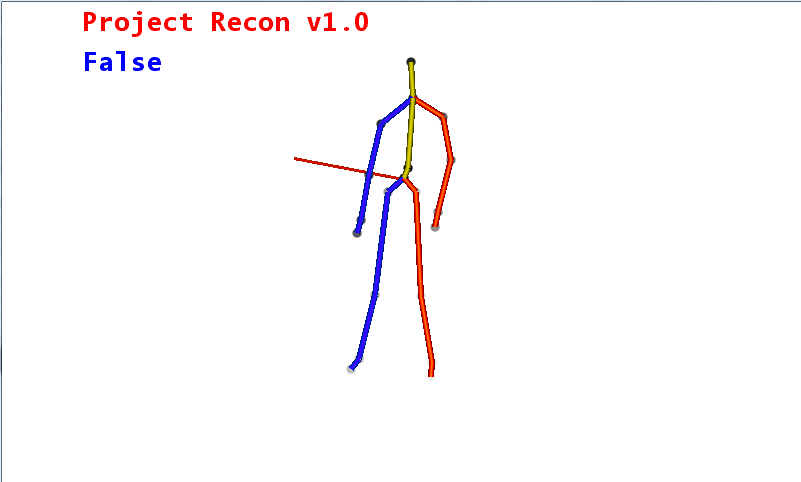
\includegraphics[width=1\textwidth]{images/skeleton_normal.png}
\caption{Skeleton with a normal vector defining where it is facing}
\label{skeletonnormal}
\end{figure}

The translation and rotation of the skeleton occurs in the Skeleton Space. The algorithm translates littleGuy to the origin point where it calculates the \N. Rotation occurs in the origin and then the new manipulated littleGuy translates back to a fixed point in the Z axis, the Y axis and X axis however remain in the origin. After this Project Recon stores the translated littleGuy in a new avatar skeleton called transGuy. The program then renders transGuy to the 2D Color Space. 
\\
The second step is using Kinect's face detection capabilities, which may be 
hard and require high processing. Errors may occur when Kinect re-swaps the joints to their right place. For this we will use the face dectetion capabilities of Kinect to create a sanity check. That is if the swap did occur and the user's face was visible, then the swap is a mistake and it will re-swap again to the correct state.
\\
When it came to testing the normalization of the skeleton using the Kinect, a problem emerges. When the user has a joint not facing the Kinect, then the Kinect does not have the position value of this joint. The reason for this is that no infrared rays are reflected from this joint. In turn, when the rotation occurs the some joints have false space(X, Y, and Z) values. This error will question the validity of the rendered and final translated values of the joints. This error made us discard this method and resort a different one that will also aims to maintain the robustness of the system.
%here talk about the final way and discuss how you will use the recognition to solve the issue with robustness 
\section{Recognition}
Recognition is the essence of this project. Recognition needs to be in real time, but most importantly how will the recognition occur. We discussed in the previous section the resolve of the normal vector. However, why is it needed? In recognition we want to be able to translate the skeleton of the person in order to always recognize from the same direction, facing the Kinect. In the coming sections we will discuss the different ways for recognition.
\subsection{Glyphs Method}
This is the proposed method in the case of recognition taking place after rotation by the help of \N as discussed earlier in this chapter. The idea behind it is to create a path taken by each joint from the skeleton and store it in an image. Creating a single image with the overall motion is and comparing it with the reference image, would be more optimal than taking a number of frames and comparing them with other reference frames.
\\
\\
As a joint moves, it creates a path shadowing its past movements. Each joint has its own exclusive color in order to differentiate if lines intersect. When the user moves the system will draw the paths taken by the joints creating some sort of a glyph image depicting the overall motion of the skeleton. An example of how a glyph would like is in both figures below. Figure 1 shows the user as he executes a move with each joint creating a path. Figure 2 shows the final glyph as it would be stored.
%image of a person with a glyph
%image with a glyph
\\
\\
After storing the glyph image, a process of image processing would take place where comparisons between the captured glyph image and the reference glyph images would begin. When a match is found, the technique would be recognized, if a match was not found the glyph image is discarded. Recognition when comparing two glyph images would of course have some sort of threshold as users are different in their executions of a technique.
\\
\\
Limitations that would emerge from using this method are the fact that motions on the z axis would be hard to recognize as the path would on the z axis wont be drawn. To solve this limitation, it is recommended that the rotation of \N around the y axis change. Rather than rotating the \N to the z axis it would rotate to form a 45$^\circ$ on the xz plane of the positive z and x axis. This way the glyph image would have a representation to motion detected on all three axes.
\\
\\
It should be clear as to when the program should record the path patterns and store the glyph. In order to know when exactly to record, we should first understand when will techniques be executed. As stated earlier, the coach gives signals to the practitioner for him to execute specific moves. Since the coach will be considered a user, it is recommended that recording of path paterns takes place as soon as a signal is initiated by the coach.
\\
\\
Since we will be unable to use the method of normalizing the skeleton due to the limitations of the Kinect sensor, this method would be obsolete in our application as the user is mobil and active around the room. Making it hard to have standard glyph patterns.

\subsection{Frames}